\documentclass{article}
\usepackage{graphicx}
\graphicspath{ {images/} }


\newcommand{\tab}[1]{\hspace{.1\textwidth}\rlap{#1}}

\begin{document}
	
\begin{titlepage}
	\newcommand{\HRule}{\rule{\linewidth}{0.5mm}} % Defines a new command for the horizontal lines, change thickness here

	\center % Center everything on the page
	 
	%----------------------------------------------------------------------------------------
	%	LOGO SECTIONS
	%----------------------------------------------------------------------------------------

	\includegraphics[width=\textwidth]{front-page}

	%----------------------------------------------------------------------------------------
	%	TITLE SECTION
	%----------------------------------------------------------------------------------------

	\HRule \\[0.4cm]
	{ \huge \bfseries Software Requirements Specification}\\[0.4cm] % Title of your document
	\HRule \\[1.5cm]
	 
	%----------------------------------------------------------------------------------------
	%	MEMBERS, TEAM NAME SECTION
	%----------------------------------------------------------------------------------------

	\begin{minipage}{0.5\textwidth}
	\begin{flushleft} \large
	\emph{Members:}\\% add your name and student here
	Peter Boxall 14056136	
	
	Orisha Orrie 13025199
	
	Nsovo Baloyi 12163262
	
	Elizabeth Bode 14310156
		
	Robert Trankle 15092454

	Nikki Constancon 15011713

	Ernst Eksteen 28398603
	\end{flushleft}
	\end{minipage}
	~
	\begin{minipage}{0.4\textwidth}
	\begin{flushright} \large
	{ \huge \bfseries Team Fuchsia }% Title of document
	{\large \today}\\
	{\large v0.1}
	\end{flushright}
	\end{minipage}\\[4cm]
\end{titlepage}


	\newpage
	
	\section{Introduction}
    	
        \subsection{Purpose}
        	{The purpose of this document is to put forth a description detailing the NavUP system. It will explain the main purpose of the system, as well as additional subsystems, the interface of these systems, and what they will and will not do, as well as the constraints. Providing a detailed requirement specification of the system as a whole. It is intended for the Client, as well as developers who will integrate the system.}
    	\subsection{Scope}
        	{NavUP will be a mobile device application, that will provide the basic functionalities of a navigation system. The system will only interoperate and function on the Hatfield main campus of the University of Pretoria.  	NavUp will provide a means to navigate the main campus of the University of Pretoria. It will thus provide users choices with regards to which routes they wish to take to reach there destination, taking into account factors such as pedestrian and vehicle traffic as well as providing routes that cater to users who may suffer physical disabilities.  NavUP's goal is to provide a personalised, efficient and convenient means of traversing the university's Hatfield campus. The system will also provide extra additional information regarding useful points of interests such as bathroom locations, as well as provide information to the user regarding the rich history of the University of Pretoria. The navigation system will be required to constantly be connected the the campus's WI-FI and will continually send up and down stream information to a server with regards to users location and destination. The server will be required to calculate the route and factor in additional information as set up by the user and there needs. The server must also be able to handle a high volume of concurrent users and provide them all with there required data. Location tracking will be achieved through the use of --WI-FI signal strength and other : not sure of exact methodology-- techniques and not through the use of GPS. /* This means that the two way communication between the device and the server must --explain requirements here-- */ }
        \subsection{Definitions, Acronyms, and Abbreviations}
        \subsection{References}
        \subsection{Overview}
	
	\section{Overall Description}
		
        \subsection{Product Perspective}
        
        	\subsubsection{System Interface}{
User Interface:
\\\\
Functionality:
\\\\
The functionality of the user interface is to allow the user to interact with the system. Through this aspect of the system the user can perform all the functions necessary to use NavUP. Through this the user is able to login and register an account, use the navigation and tracking systems as well as well as view map information and become apart of the gamification of the application.
\\\\
How functionality achieves requirements:
\\\\
The user interface allows the functionality of the application to meet the requirements. The user is able to navigate to the necessary location through searching and navigating via this UI, fulfilling the navigation requirement. The user is able to be displayed information of disability access, generic map information and even receive notifications through this UI, fulfilling these requirements. 
\\\\
Hardware Interface:
\\\\
Functionality:
\\\\
The functionality of this system interface is the physical hardware that allows software operation. The hardware in this case is specifically the mobile devices upon which the NavUP application will be installed.
\\\\
How functionality achieves requirements :
\\\\
This hardware will allow the achievement of the requirements by facilitating the operation of the application. The user will be able to press the physical device screen in order to operate the navigation and other such features of the application. The networking hardware of the components such as the wireless fidelity infrastructure within the device allows for communication to the system server. It is through this communication that the user's location can be determined and the system can function.
\\\\
Software Interface:
\\\\
Functionality:
\\\\
The functionality of the software interface is to facilitate the communication between the hardware infrastructure of the devices running the application and the actual NavUP application. An example of this would be the operating system of the device in use. The operating system would allow the application to make use of the wifi infrastructure and communicate the necessary information to the application. This would enable the device to communicate with the server and perform the necessary requests.
\\\\
How functionality achieves requirements :
\\\\
This would allow the achievement of the requirements as the communication of the application to the system server is vital to the operation of the NavUP system. By allowing communication over wifi the user's location can be determined, accounts can be logged in or created, information regarding heat mapping and general information can be retrieved by the user, fulfilling this requirement. Notifications can also be received by the users application through the wifi communication , fulfilling the this requirement .}

		
            \subsubsection{User Interface}
	    {All users will have access to the navigation system when the application is launched.
They will be able to enter a destination and follow the path to location/lecture hall specified(see Figure 1).
The users will also be able to select preferences such as disability access path, which will enable them to travel the path with ease.\\\\
The users will be able to view information each building, giving them additional historic information about the building(Figure 2). If they do not not wish to 
view information about the building, they must simply not click on the information symbol available.
They will also be allowed to view each room. The navigation system will allow the users to select points of interest, such as food dispensaries, 
smoking locations, and toilets. They will be able to turn on and off indicators for these points of interest.
The users may access a view to heat paths on the map, to show an increase in crowd population in a dense area.\\\\
For the account user interface, the registered students and employees will be able to login to their account, using their clickUP information.
There will be certain accounts with administrative privileges that will be able to create and delete accounts, as deemed necessary.\\\\
The application will be able to send users notifications, on events that occur on campus as well as a report of information, such as the amount of 
steps walked per week. Students and employees will be able to remove push notifications, if they do not wish to receive them from the system.\\\\
}
\begin{figure}[h]
\centering
\begin{minipage}{.5\textwidth}
	\centering
	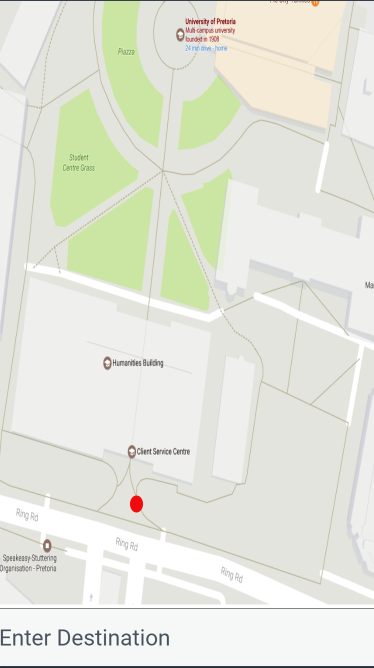
\includegraphics[width=2cm, height 8cm]{Navigation}
	\caption{Navigation System}
\end{minipage}%
\begin{minipage}{.5\textwidth}
	\centering
	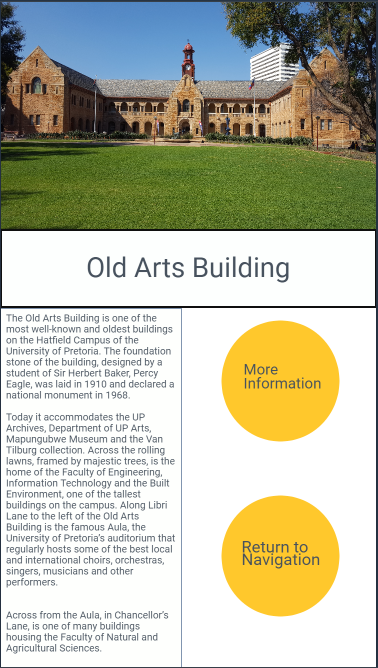
\includegraphics[width=2cm, height 8cm]{BuildingInfo}
	\caption{Building Information}
\end{minipage}%
\end{figure}


            \subsubsection{Hardware Interface}
		{
			There will be a hardware interface with the routers across the campus in order to triangulate the position of the user and to create heatmaps. The actual Wi-Fi interface between the phone and Wi-Fi will be abstracted by the phone and will be managed by the actual underlying operating system on the phone.}
            \subsubsection{Software Interface}
            \subsubsection{Communications Interface} \begin{itemize}
	    \item Users using the web will use HTTP/HTTPS protocol.
	    \end{itemize}
            \subsubsection{Memory}
	    {The mobile application will use a significant amount of space, roughly 300MB, which is due to graphics as well as the mobile application being able to use Wi-Fi as well as GPS to navigate it's location.\\
Primary memory(RAM) will use 200MB on average, based on how long the application is being used.}
            \subsubsection{Operations}
            	{The user will require a series of normal and special case operations to be fulfilled by the system. The user will use the system in normal case operations that comprise of finding the users location, finding a location the user is interested in, including locations such as toilets, and navigating, tracking and guiding the user to these locations. The user will also use the system to save locations of interest for future use as well as check extra information for improved path finding, such as pedestrian traffic, distance or vehicle traffic.\\\\
            	The system will consist of three modes of operation. One  being a general case of functionality, available to all users, that provides wayfinding capabilities to all users of the system. The other being a logged in operational mode which allows access to additional features such as account management, route sharing and rating and data storage. The final mode being a special mode of operation that will be an administrative mode. This mode allows the user to generate and manage events, update and maintain the system as well as generate notifications that will be received by other users.\\\\
            	Special modes of operation will involve the system pushing user specific information to the user device that may interest them or might require a route recalculation by the system due to environmental changes, such as pedestrian traffic flow or event related locations of interest as set out by the administrative user. Another special mode of operation is the systems ability to generate interesting facts for the user about locations found on campus, which will be useful to generals users who have an interest in history, while not being intrusive to users who do not care for the operation.\\\\
            	The general user will primarily use the system in en-route to various locations. This will primarily take place between periods of the University time table. Other periods will primarily see the system being used by students with an off period or by visitors and lecturers. The system will see unattended periods of operations while a user is actually walking and being tracked by the system. Further unattended periods of operations will occur when the Server pushes relevant data regarding events and user preferences to the user device.\\\\
            	The user will be able to view live heat maps of the main campus which allow them to gauge where the most pedestrian traffic is and avoid those routes. The system will also provide a mode which highlights features such as wheelchair ramps and other facilities that enable an easier means of navigating the campus. The system will by default select routes that it has calculated to be the most direct, however the user may choose to set the route navigation into other modes which select the highest ranked routes, the scenic routes or the users saved routes. Points of interest can also be searched for and ordered and filtered by rating and distance.\\\\
            	The system will provide a registered user the option to either save there data, such as preferences, locally on the device or remotely on the server. The system will also provide administrative users methods for backing up the system and several different forms of readouts, reports and tabulations regarding the state and use of the system which can be gathered at an annual or intermittent period and backed up for analysis.}
            \subsubsection{Sit Adaption Requirements}
        
		\subsection{Product Functions} {The main function of the NavUP system will be to show students how to get around campus in the shortest possible way. Thus, this will entail using WiFi, mobile networks and possibly GPS to navigate around Hatfield campus. The basic functions will include:  }
	\begin{itemize}
  		\item A heat map to show pedestrian traffic.
		\item Providing the shortest path from point A to point B.
 		 \item A distance tracker to show users the distance left until they reach their destination.
		\item A specialized route for disabled users.
		\item Points of interest around the university such as restaurants, ATMs, the church, Scienza and Botanical Gardens.
 		 \item Essential Areas such as bathrooms, parking areas and smoking areas.
		\item Exact locations of buildings as well as the lecture halls that they consist of.
		\item A "Where am I?" function to show users exactly what is around them.
 		 \item Historical backgrounds of buildings and different parts of campus.
		\item A login page for users who would like access to more of the personalised functions. Theses functions will be saving locations for future use, a game which rewards users when they reach a certain distance and saving user preferences and interests.
		\item A random facts generator for distance rewards.
		\item Switching between Wi-Fi, mobile data and GPS to navigate around campus.
		\item A timetable function for users to input their timetables and show exactly where their lectures will take place with reminders.
		\item Provide administrative security for login functionality.
		\item Rating system and review for restaurants and parking.
		\item Route options such as scenic routes and fastest route.
		\item Ability to share directions as well as estimated time of arrival.
	\end{itemize}
    	\subsection{User Characteristics}  
		{ 

There will be three main types of users interacting with the system, namely a general user, a registered user and an admin. Each of these types will have different rights and access to the system and thus their own requirements.\\\\}

{The general user will use the system to navigate from their location to another specified location. They will need minimal skill in order to utilise the application, including the ability to connect to the Wi-Fi and indicate intended location. The general user will have restricted usage of the in-app game and certain privileges that require a user profile. They will not require any additional expertise or education to function the application.\\\\}

{The registered user will have the same access as the general user plus access to the in-app game and more personilized search options. They will not require any technical skills sans the ones mentioned for the general user. They will also require minimal expertise and education since the app will be designed for easy to understand user interaction.\\\\}

{The Adimin user will require additional permissions in order to create events and update information. They will need a higher level of expertise to manage and collect information on up-coming and relevant events. They will need minimal education but rather a general knowledge of the campus and the history of the campus. Their technical skill must include the ability to use the application functions to add and edit information and events.\\\\} 
    	\subsection{Constraints}   
    	\subsection{Assumptions and Dependencies}

	\section{Specific Requirements}
    
    	\subsection{External Interface Requirements}
    	\subsection{Functional Requirements}
	{
	\begin{center}
\textbf{UI: Find Current Location}
\begin{tabular}{ |p{7cm}|p{7cm}| } 
 \hline
 Actor: General User & System: Navigation\\ 
\hline \hline
 & 0: System displays map on main page\\ 
\hline
 1:TUCBW General User clicks on "Find current location" button & 2: System displays search bar with the location name as well as a pin on the location \\ 
\hline
3: General user confirms that it has the correct location & \\
 \hline
\end{tabular}
\end{center}


\begin{center}
\textbf{UI: Get Directions To Location}
\begin{tabular}{  |p{7cm}|p{7cm}| } 
 \hline
 Actor: General User & System: Navigation\\ 
\hline \hline
 & 0: 0: System displays map on main page\\ 
\hline
 1:TUCBW General User clicks on "Find location" button & 2: System displays search bar \\ 
\hline
3: User types in intended location & 4: System displays map with pinned location \\
 \hline
5: User clicks on "Navigate To" button & 6:System asks user to input starting location \\
 \hline
7: User inputs starting location & 8:System searches for starting location \\
 \hline
9: User selects confirm button & 10: System displays map to location \\
 \hline
11: User follows directions &  \\
 \hline
\end{tabular}
\end{center}
	
\noindent\textbf{UC: Track User Location}
\begin{flushleft}
\begin{tabular}{ |p{0.5\textwidth}|p{0.5\textwidth}| }
  \hline
  \multicolumn{2}{|p{\textwidth}|}{\textbf{Precondition:} The user must have followed the steps to get directions from their current location to a specified location} \\
  \hline
  \textbf{Actor: General User}  & \textbf{System: Navigation} \\
   \hline
   & 0. The system displays the campus map indicating users chosen route. \\
  \hline
  1. TUCBW general user clicks the Start Navigation button on the map page& 2. The system displays sets of directions until the user arrives at their specified location or they terminate the instruction\\
  \hline
  3. User follows the sets of directions as they are displayed until they reach their chosen destination& 4. The system notifies the user that the destination has been reached\\
  \hline
  5. TUCEW the general user confirms that the destination has been reached& \\
  \hline
  \multicolumn{2}{|p{\textwidth}|}{\textbf{Postcondition: None}} \\
   \hline
\end{tabular}
\end{flushleft}

\bigskip
\bigskip

\noindent\textbf{UC: View Traffic}
\begin{flushleft}
\begin{tabular}{ |p{0.5\textwidth}|p{0.5\textwidth}| }
  \hline
  \multicolumn{2}{|p{\textwidth}|}{\textbf{Precondition:} The user must have followed the steps to get directions from their current location to a specified location} \\
  \hline
  \textbf{Actor: General User}  & \textbf{System: Navigation} \\
   \hline
   & 0. The system displays the campus map indicating users chosen route. \\
  \hline
  1. TUCBW general user selects the option to display traffic en-route & 2. The system updates the displayed map to indicate highly congested area in red\\
  \hline
  3. TUCEW the general user sees the areas of high congestion marked on the map in red.&\\
  \hline
  \multicolumn{2}{|p{\textwidth}|}{\textbf{Postcondition: None}} \\
   \hline
\end{tabular}
\end{flushleft}
}
        \subsection{Performance Requirements}
	{Performance requirements bullet list:\\\\
One can segregate the performance requirements of the Nav-UP system up into two components. These two components are:\\\\
1. User -Client Application Performance requirements\\\\
This component of the system with specific regards to performance requirements is all aspects of performance relating to the user experience on the client-side. This refers to the user experience with regards to mobile application operation or web client operation.\\\\
2. System- Server Performance Requirements\\\\
This component of the system, with specific regards to the performance requirements, is all aspects involved with communication and operation on a server level. This refers to all interactions with the server running Nav-UP.\\\\
Client Application Requirements\\\\
1.	Software needs to be responsive and lightweight enough to run on mobile hardware.\\\\
2.	The networking aspect of the software should not hamper the UI thread of the application while in use to ensure a smooth user experience.\\\\
3.	During User navigation the Navigation system will need to perform in real time showing turns as taken and arrival as necessary.\\\\
4.	The data usage should be kept to a minimum as to not overload the campus Wi-Fi infrastructure being used for non-navigational purposes.\\\\
Server Performance Requirements\\\\
1.	The system has to be able to handle a capacity of around 30, 000 concurrent users sending, receiving and processing information.\\\\
2.	The system storage capacity should be able to scale to the information retention of 30 000 accounts and locations and be able to retrieve them in a timely manner.\\\\
3.	The System will need to be able to concurrently handle account creation.\\\\
4.	The system should be able to calculate and display a heat-map in the correct timing as to ensure an as accurate shortest path calculation as possible for user navigation.\\\\

	}
        \subsection{Design Constraints}
        \subsection{Software System Attributes}
		{		
			The software system will have the following attributes:
\\\\
		Availability: The system and its functions will be available across campus as long as there is an Internet connection with the campus Wi-Fi. 
\\\\
		Reliability: The system will provide directions to the correct location, from the correct location, consistently. The system will always be up-to-date and will give correct reliable information regarding the campus and the events on the campus.
\\\\
		Portability: The system will be able to function across a multitude of interfaces. Therefore, it will be able to port between Android and iOS with ease. 
\\\\
		Maintainability: The application will be able to be extended easily with new functionality. There will also be a good test environment to reduce an make it easy to find system errors.  
\\\\
		Security: The system will guarantee security of the users personal login information. It will also keep the preferences collected from the user secure and private. The Admin will also have a secure login account to prevent unauthorized access.}
        \subsection{Other Requirements}
	
	\section{Vision}


	\section{Background}
	
\end{document}
